\section{Miscellanea}

\subsection{Heterogeneous Aspect}

In addition to the Built-In Aspect, we are architecting a novel variant, termed as the Heterogeneous Aspect, to facilitate heterogeneous computing on the blockchain. Heterogeneous computing implies native applications cultivated based on operating systems, thus exploiting operating system resources, network requests, and an array of software utilities to construct sophisticated application logic. Presently, heterogeneous computing is primarily achieved via off-chain computations, including off-chain oracles.

This design addresses the inherent limitations of the Built-in Aspect. Operating within a virtual machine, the Built-in Aspect necessitates deterministic execution, resulting in confined resource access. On the other hand, the Heterogeneous Aspect is granted network access, enabling it to undertake demanding computational tasks. For example, running AI models, which are resource-intensive and yield non-deterministic execution results, might not be viable on virtual machines. However, these tasks are feasible within the Heterogeneous Aspect's framework.

The Heterogeneous Aspect, inherently a native application, is encapsulated within containers. This approach affords an expansion in the technological repertoire of the decentralized sphere by integrating advancements such as artificial intelligence, privacy computation, real-time computation, and decentralized storage. Heterogeneous Aspect's deployment and execution are handled within a heterogeneously architected computing network, a network that shares security in mutual accordance with the main network.

The differences between Built-in Aspects and Heterogeneous Aspects are shown in the table:

\begin{table}[htbp]
    \centering
    \begin{tabular}{|l|p{6cm}|p{6cm}|}
      \hline
      & Built-in Aspect & Heterogeneous Aspect \\
      \hline
      Consensus mechanism & Loaded and executed by main net validator nodes & Can be executed by heterogeneous computing nodes, and shares security with main net validation nodes \\
      \hline
      Execution environment & Executed in a deterministic sandbox environment & Supports interaction with external heterogeneous computing platforms and external networks \\
      \hline
      Runtime restrictions & Provides limited Runtime APIs, no IO/thread/async operation/network and other high-uncertainty operation capabilities & Native program, not limited by its execution capabilities \\
      \hline
    \end{tabular}
  \end{table}
  


\subsection{Difference Between Aspect and Off-chain Computation}

Off-chain computation refers to a model similar to Oracle, where computations occur on an off-chain consensus network. The consensus is reached off-chain on the calculated results before these are input into smart contracts for utilization.
The distinctions between Aspect and off-chain computation encompass:

\begin{itemize}
  \item \textbf{Security:} Relative to L1, the contrast between Aspect and off-chain computation parallels the differences between rollup and side-chain. While one shares security with the main network, the other assumes responsibility for its security.
  \item \textbf{Interoperability:} Both Aspect and off-chain computation exhibit interoperability with contracts on L1, similar to the interoperability seen within intra-chain contract interactions and across different chains. Aspect and contract execution occur synchronously within the same transaction, whereas off-chain computation and contracts establish a distributed transaction and are typically asynchronous.
  \item \textbf{Characteristics:} As an on-chain native program, Aspect forms part of the consensus process. It can operate within the context of the consensus execution process, such as customizing transaction data structures, validating methods, and appending additional transactions.
\end{itemize}

In conclusion, Aspect and off-chain computation can act as synergistic complements to each other, empowering both smart contracts and applications. However, due to its native extension features, Aspect possesses unique functionalities that off-chain computation cannot replicate.

\subsection{About Latency Problem}

Transactions executing both a smart contract and an Aspect may exhibit elevated latency in comparison to those executing a smart contract alone. It is critical to distinguish between the following two scenarios:

\begin{enumerate}
  \item \textbf{Embedding a specific logic in an Aspect for an existing smart contract.} In the absence of an Aspect, this particular logic could be executed within off-chain components, thus not contributing to increased on-chain latency. However, if we shift this logic from off-chain components to on-chain Aspects, the transaction latency would escalate.
  \item \textbf{Implementing specific functionality via an EVM-based smart contract augmented by a WASM-based Aspect.} Were this specific functionality to be implemented exclusively by the EVM-based smart contract, transaction calls to this functionality would exhibit increased latency, as the WASM-based Aspect executes at a faster rate than the smart contract. In this scenario, the Aspect mitigates the latency.
\end{enumerate}

Despite these two scenarios seemingly contradicting each other, it is a fallacy to assume that Aspects inherently increase latency. The latency is predominantly determined by the transaction's gas limit. Given the same latency, transactions executed through an Aspect can utilize more gas.

To elucidate the computational overhead inherent to Aspect and discern the equilibrium between the EVM and ArtWASM computational costs, a series of tests were constructed, leveraging the canonical Fibonacci algorithm.

The experimental conditions were as follows:

\begin{enumerate}
  \item The ArtWASM runtime is instantiated in Go, with WASMTime functioning as the execution engine.
  \item The test bed comprised a system equipped with a 2.2 GHz Haswell CPU.
  \item The deployed smart contract was formulated using Solidity version 0.8.20, juxtaposed with the Aspect test code contrived via Assembly Script 0.27.5.
  \item Compilations in both Solidity and Assembly Script were devoid of optimizations, ensuring the Aspect code compilation via the -O0 flag. Subsequent validation was performed on the resultant .wat file to confirm the absence of compiler optimizations.
\end{enumerate}

In the first experiment, with join-points capped at 10, Fibonacci computation iterations were sequentially incremented. This scheme aimed to discern the computational threshold where Aspect's efficiency supersedes that of a traditional smart contract.

\begin{figure}[htp]
  \centering
  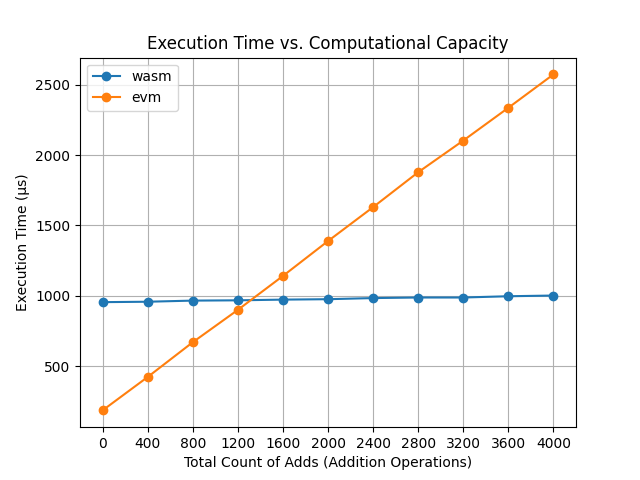
\includegraphics[width=0.5\textwidth]{sections/tx-latency-et-vs-cc.png}
  \caption{Equilibrium Analysis between Aspect and Smart Contract Computation}
\end{figure}

Given Fibonacci(0) incurs zero computational overhead, the duration is solely attributed to context switches. From the Fibonacci(0) execution time, the context switch durations (in microseconds) for ArtWASM and EVM are deduced as:

\begin{align*}
  95.5 &= \frac{955}{10} \\
  18.6 &= \frac{186}{10} \\
\end{align*}

Thus, the computational costs for ArtWASM and EVM are delineated as:

\[
\text{ArtWASM Execution Cost} \equiv 95.5 \times \text{Number of Join Points} + \text{Execution Cost}
\]
\[
\text{EVM Execution Cost} \equiv 18.6 \times \text{Number of Calls} + \text{Execution Cost}
\]

A detailed analysis of Ethereum block gas yields an average transactional gas consumption approximating 280,079.07. This aligns closely with the gas requisites for Fibonacci(1600), 280,255. Assuming Fibonacci(1600) execution times for ArtWASM and EVM are denoted by \(x\) and \(y\) microseconds respectively, the equations become:

\begin{align*}
973 &= x + 955 \\
1141 &= y + 186 \\
\end{align*}

Resolving this system furnishes \(x = 18\) and \(y = 955\). Concurrently, this facilitates the calculation of the performance differential between ArtWASM and EVM:

\[
  \frac{\text{EVM Execution Cost}}{\text{ArtWASM Execution Cost}} \equiv \frac{955}{18} \approx 53
\]

This demonstrates an approximate 52 times faster in ArtWASM's computational prowess relative to EVM for standard Ethereum transaction computations.

In a subsequent test, 1600 Fibonacci iterations were executed on both EVM and ArtWASM. The configuration was attuned to iteratively augment the number of join-points, thereby enabling a correlation analysis between ArtWASM and EVM execution times.

\begin{figure}[htp]
  \centering
  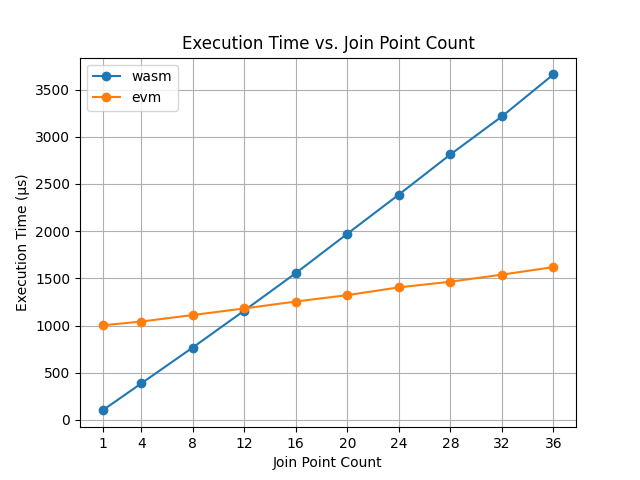
\includegraphics[width=0.5\textwidth]{sections/tx-latency-et-vs-jpc.png}
  \caption{Performance Interrelation between ArtWASM and EVM}
\end{figure}

The depicted correlations suggest that for generic Ethereum transaction computations, exceeding 12 join-points drastically diminishes the computational advantages offered by Aspect, primarily due to context switching overheads. Hence, Artela's optimal join-point threshold is posited at 12.

To more precisely sculpt the Aspect specification in line with typical usage paradigms, we have made the following assumptions:

\begin{enumerate}
  \item A minority of join-points will be actualized by Aspects, averaging to approximately 3 per implementation.
  \item The computational overhead per join-point is projected to align closely with traditional smart contracts.
  \item Typically, an individual smart contract will bind to an average of 3 Aspects.
\end{enumerate}

Given the empirical data and derived formulas, Artela's gas limit is postulated as:

\[
  \text{AvgTxGasLimit} \equiv (\frac{\text{AvgJoinPoints} \times \text{AvgAspectsBound} \times (\text{AvgContextSwitch} + \text{AvgExecution})}{\text{AvgTxTime}} + 1) \times \text{AvgTxGas}
\]

\[
  \text{AvgTxGasLimit} \equiv (3 \times 3 \times (95.5 + 18) / 1002 + 1) \times  \text{AvgTxGasCost} \approx 1.019 \times \text{AvgTxGasCost}
\]

From the above formula, Artela's enhanced computational latitude becomes manifest. While there's an uptick of approximately 101.9\% in gas limit, the computational allowance increases 900\%, equipping developers to conceive dApps with way more complexity, at a marginal 101.9\% latency escalation. The current block gas limit of Ethereum is about 30,000,000, so a reasonable block gas limit for integrating Aspect will be 60,580,000.

In summary, the integration of Aspect functionality affords Artela's blockchain the capacity to embrace elevated gas limits relative to other EVM-compatible blockchains. To fully harness Aspect's potential and bolster the transaction gas limit, Artela is architected to advocate for parallel transaction execution, inherently trimming latency.